\documentclass[12pt]{article}
 
\usepackage[margin=1in]{geometry}
\usepackage{amsmath,amsthm,amssymb}
\usepackage{mathtools}
\DeclarePairedDelimiter{\ceil}{\lceil}{\rceil}
%\usepackage{mathptmx}
\usepackage{accents}
\usepackage{comment}
\usepackage{graphicx}
\usepackage{IEEEtrantools}
 \usepackage{float}
 
\newcommand{\N}{\mathbb{N}}
\newcommand{\Z}{\mathbb{Z}}
\newcommand{\R}{\mathbb{R}}
\newcommand{\Q}{\mathbb{Q}}
\newcommand*\conj[1]{\bar{#1}}
\newcommand*\mean[1]{\bar{#1}}
\newcommand\widebar[1]{\mathop{\overline{#1}}}


\newcommand{\cc}{{\mathbb C}}
\newcommand{\rr}{{\mathbb R}}
\newcommand{\qq}{{\mathbb Q}}
\newcommand{\nn}{\mathbb N}
\newcommand{\zz}{\mathbb Z}
\newcommand{\aaa}{{\mathcal A}}
\newcommand{\bbb}{{\mathcal B}}
\newcommand{\rrr}{{\mathcal R}}
\newcommand{\fff}{{\mathcal F}}
\newcommand{\ppp}{{\mathcal P}}
\newcommand{\eps}{\varepsilon}
\newcommand{\vv}{{\mathbf v}}
\newcommand{\ww}{{\mathbf w}}
\newcommand{\xx}{{\mathbf x}}
\newcommand{\ds}{\displaystyle}
\newcommand{\Om}{\Omega}
\newcommand{\dd}{\mathop{}\,\mathrm{d}}
\newcommand{\ud}{\, \mathrm{d}}
\newcommand{\seq}[1]{\left\{#1\right\}_{n=1}^\infty}
\newcommand{\isp}[1]{\quad\text{#1}\quad}

\DeclareMathOperator{\imag}{Im}
\DeclareMathOperator{\re}{Re}
\DeclareMathOperator{\diam}{diam}
\DeclareMathOperator{\Tr}{Tr}

\def\upint{\mathchoice%
    {\mkern13mu\overline{\vphantom{\intop}\mkern7mu}\mkern-20mu}%
    {\mkern7mu\overline{\vphantom{\intop}\mkern7mu}\mkern-14mu}%
    {\mkern7mu\overline{\vphantom{\intop}\mkern7mu}\mkern-14mu}%
    {\mkern7mu\overline{\vphantom{\intop}\mkern7mu}\mkern-14mu}%
  \int}
\def\lowint{\mkern3mu\underline{\vphantom{\intop}\mkern7mu}\mkern-10mu\int}




\newenvironment{theorem}[2][Theorem]{\begin{trivlist}
\item[\hskip \labelsep {\bfseries #1}\hskip \labelsep {\bfseries #2.}]}{\end{trivlist}}
\newenvironment{lemma}[2][Lemma]{\begin{trivlist}
\item[\hskip \labelsep {\bfseries #1}\hskip \labelsep {\bfseries #2.}]}{\end{trivlist}}
\newenvironment{exercise}[2][Exercise]{\begin{trivlist}
\item[\hskip \labelsep {\bfseries #1}\hskip \labelsep {\bfseries #2.}]}{\end{trivlist}}
\newenvironment{problem}[2][Problem]{\begin{trivlist}
\item[\hskip \labelsep {\bfseries #1}\hskip \labelsep {\bfseries #2.}]}{\end{trivlist}}
\newenvironment{question}[2][Question]{\begin{trivlist}
\item[\hskip \labelsep {\bfseries #1}\hskip \labelsep {\bfseries #2.}]}{\end{trivlist}}
\newenvironment{corollary}[2][Corollary]{\begin{trivlist}
\item[\hskip \labelsep {\bfseries #1}\hskip \labelsep {\bfseries #2.}]}{\end{trivlist}}

\newenvironment{solution}{\begin{proof}[Solution]}{\end{proof}}
 
\begin{document}
 
% --------------------------------------------------------------
%                         Start here
% --------------------------------------------------------------
\title{Math 115A Homework 2}
\author{Ethan Martirosyan}
\date{\today}
\maketitle
\hbadness=99999
\hfuzz=50pt
\section*{Problem 1}
The number of lattice points in this region can be found by counting the number of lattice points between $0$ and $f$ at each integer $m$ between $Q$ and $R$ and adding these numbers. The number of lattice points between $0$ and $f$ at an arbitrary integer $m$ is equal to the number of positive integers less than or equal to $f(m)$. By the definition of the floor function, we find that the number of lattice points between $0$ and $f$ at $m$ is equal to $[f(m)]$. Summing this over all integers $m$ between $Q$ and $R$, we find that the number of lattice points in this region is equal to
\[
\sum_{Q < n \leq R} [f(n)]
\]
\newpage
\section*{Problem 2}
First, we note that the sum
\[
\sum_{0<m<Q/2} \bigg[\frac{P}{Q}m \bigg]
\] is equal to the number of lattice points $(x,y)$ satisfying $0<x\leq Q/2$ and $0<y \leq Px/Q$. That is, it is equal to the cardinality of the set
\[
S_1 = \{(x,y)\in \mathbb{Z} \times \mathbb{Z}: 0<x\leq Q/2,\; 0<y \leq Px/Q\}
\] This is true because for every integer $x$ between $0$ and $Q/2$, we count $[Px/Q]$ lattice points, which is the number of positive integers $y$ less than $Px/Q$. Geometrically, $S_1$ is the blue triangle in the image on the next page. Next, we note that the sum
\[
\sum_{0<n<P/2} \bigg[\frac{Q}{P}n \bigg]
\] is the number of lattice points $(x,y)$ satisfying $0<y\leq P/2$ and $0<x\leq Qy/P$. That is, it is equal to the cardinality of the set
\[
S_2 = \{(x,y) \in \Z \times \Z: 0<y\leq P/2,\; 0<x \leq Qy/P\}
\] This is because for every integer $y$ satisfying $0<y\leq P/2$, we count $[Qy/P]$ lattice points, which is the number of positive integers $x$ less than $Qy/P$. Geometrically, $S_2$ is the red triangle in the image on the next page. Finally,
\[
\frac{P-1}{2} \cdot \frac{Q-1}{2}
\] is the number of lattice points $(x,y)$ such that $0<x\leq Q/2$ and $0<y\leq P/2$ or the cardinality of the set
\[
S_3 = \{(x,y) \in \mathbb{Z} \times \mathbb{Z}: 0 < x \leq Q/2,\; 0 < y \leq  P/2\}
\] This is true because $P$ and $Q$ are both assumed to be odd. Geometrically, $S_3$ is the union of the red and blue triangles in the image on the next page, so the result is intuitively clear. Now, we must prove this rigorously. We claim that $S_3 = S_1 \cup S_2$ and $S_1 \cap S_2 = \varnothing$. First, we will prove that $S_3 = S_1 \cup S_2$. Let us suppose that $(x,y) \in S_3$. Then, we know that $0 < x \leq Q/2$ and $0 < y \leq P/2$. For the sake of contradiction, let us suppose that $(x,y) \not \in S_1 \cup S_2$. This implies that $y > Px/Q$ and $x > Qy/P$. This yields $Qy > Px$ and $Px > Qy$ so that $Qy > Px > Qy$, a contradiction. Thus we may deduce that $(x,y) \in S_1 \cup S_2$ so that $S_3 \subseteq S_1 \cup S_2$. Next, we may suppose that $(x,y) \in S_1 \cup S_2$. Then, we know that $(x,y) \in S_1$ or $(x,y) \in S_2$. If $(x,y) \in S_1$, then we have $0 < x \leq Q/2$ and $0 < y \leq Px/Q \leq (P/Q)(Q/2) = P/2$, so $(x,y) \in S_3$. If $(x,y) \in S_2$, then we have $0 < y  \leq P/2$ and $0 < x \leq Qy/P \leq (Q/P)(P/2) = Q/2$ so that $(x,y) \in S_3$. Thus, we may deduce that $S_1 \cup S_2 \subseteq S_3$ so that $S_1 \cup S_2 = S_3$. Next, we will show that $S_1 \cap S_2 = \varnothing$. For the sake of contradiction, suppose that there was some $(x,y) \in S_1 \cap S_2$. Then we would know that $0 < y \leq Px/Q$ and $0 < x \leq Qy/P$. This yields $Qy \leq Px$ and $Px \leq Qy$ so that $Px = Qy$. Then, we find that $P \mid Qy$. Since $(P,Q)=1$ by assumption, we realize that $P \mid y$. This is impossible since $y < P/2$. Thus, we may deduce that $S_1 \cap S_2 = \varnothing$. Now, we may write
\[
\frac{P-1}{2} \cdot \frac{Q-1}{2} = \vert S_3 \vert = \vert S_1 \cup S_2 \vert = \vert S_1 \vert + \vert S_2 \vert = \sum_{0<m<Q/2} \bigg[\frac{P}{Q}m \bigg] + \sum_{0<n<P/2} \bigg[\frac{Q}{P}n \bigg] 
\]
\begin{figure}[H]
\centering
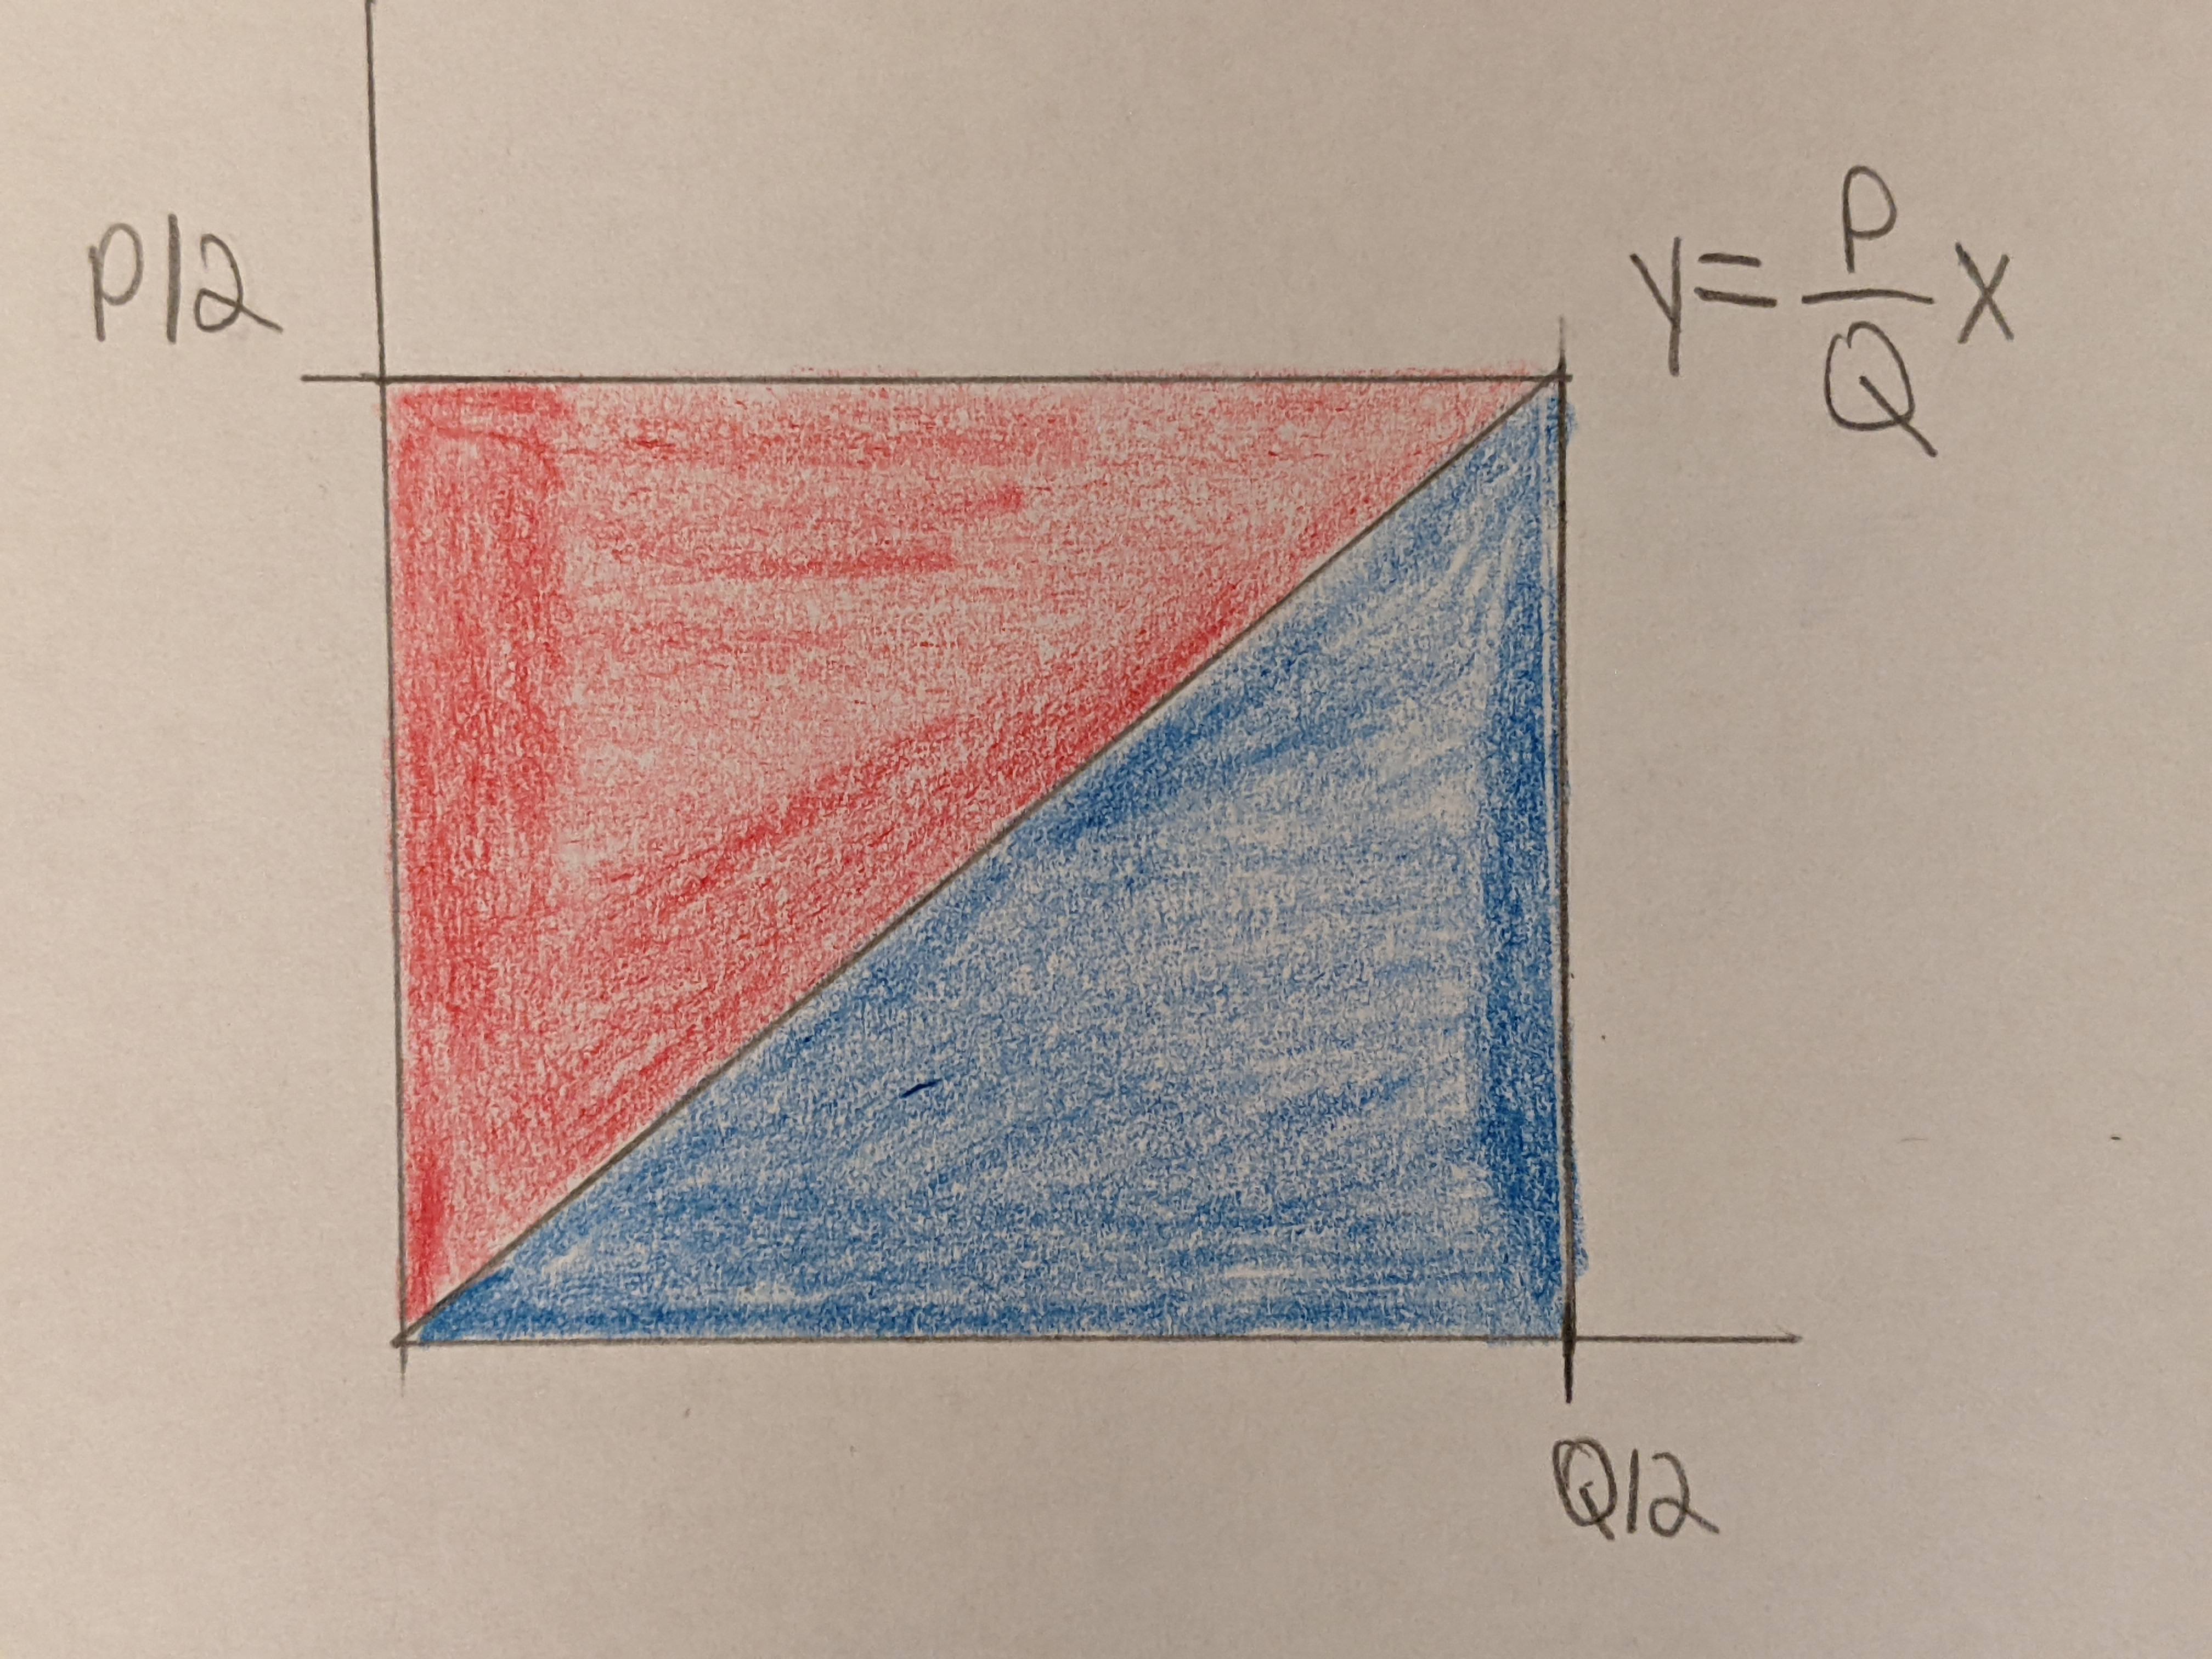
\includegraphics[width=\textwidth]{Problem2Image1}
\end{figure} 
\newpage
\section*{Problem 3}
By the division algorithm, we may write $[\alpha] = cq + r$, where $0 \leq r \leq c-1$. Now, we may note that
\[
\bigg[ \frac{[\alpha]}{c}\bigg] = \bigg[ \frac{cq+r}{c}\bigg] = \bigg[ q+ \frac{r}{c} \bigg] = q
\] because $r < c$. Next, we know that $\{\alpha\} = \alpha - [\alpha]$ so that $\alpha = [\alpha] + \{\alpha\}$. Thus, we find that
\[
\bigg[\frac{\alpha}{c}\bigg] = \bigg[\frac{[\alpha] + \{\alpha\}}{c}\bigg] = \bigg[\frac{ cq + r + \{\alpha\}}{c}\bigg] = \bigg[ q + \frac{r+\{\alpha\}}{c}\bigg] = q
\] because $0 \leq \{\alpha\} < 1$ and $r \leq c - 1$ so that $r+\{\alpha\} < c$.
\newpage
\section*{Problem 4}
By Problem $3$, we may suppose without loss of generality that $X$ is an integer. In class, we proved that
\[
\sum_{n \leq X} f(n) \bigg[ \frac{X}{n} \bigg] = \sum_{n \leq X} g(n)
\] where $f$ is an arithmetic function and $g$ is the mobius transform of $f$. Let us take $f \equiv 1$; that is, $f$ is identically $1$. Then
\[
g(n) = \sum_{d\mid n} f(d) = \sum_{d\mid n} 1 = \tau(n)
\] since $\tau$ counts the number of positive divisors of $n$. Substitution then yields
\[
\sum_{n \leq X} \bigg[ \frac{X}{n} \bigg] = \sum_{n \leq X} f(n) \bigg[ \frac{X}{n} \bigg] = \sum_{n \leq X} g(n) = \sum_{n \leq X} \tau(n)
\] 
\newpage
\section*{Problem 5}
By Problem $3$, we may suppose without loss of generality that $X$ is an integer. By problem $4$, we know that
\[
\sum_{n \leq X} \tau(n) = \sum_{n\leq X} \bigg[\frac{X}{n}\bigg]
\] Therefore, we only have to show that
\[
\sum_{n\leq X} \bigg[\frac{X}{n}\bigg] = 2 \sum_{n \leq \sqrt{X}} \bigg[\frac{X}{n}\bigg] - [\sqrt{X}]^2 
\] Notice that
\[
\sum_{n\leq X} \bigg[\frac{X}{n}\bigg]
\] represents the cardinality of the set
\[
T = \{(a,b) \in \Z \times \Z: 0 < a \leq X,\; 0 < b \leq X/a\}
\] In the image below, $T$ is the union of the blue, green, and red regions. Furthermore, 
\[
\sum_{n \leq \sqrt{X}} \bigg[\frac{X}{n}\bigg]
\] represents the cardinality of the set
\[
U = \{(a,b) \in \Z \times \Z: 0 < a \leq \sqrt{X},\; 0 < b \leq X/a\}
\] In the image below, $U$ is the union of the blue and green regions. Furthermore,
\[
\sum_{n \leq \sqrt{X}} \bigg[\frac{X}{n}\bigg]
\]
also represents the cardinality of the set
\[
W = \{(a,b) \in \Z \times \Z: 0 < b \leq \sqrt{X},\; 0 < a \leq X/b\} 
\] In the image below, $W$ is the union of the green and red regions. Finally, we may note that $[\sqrt{X}]^2$ represents the cardinality of the set
\[
V = \{(a,b) \in \Z \times \Z: 0 < a \leq \sqrt{X},\; 0 < b \leq \sqrt{X}\}
\]
 In the image below, $V$ is the green region. From this image, it is clear that counting all the lattice points in $T$ is equivalent to adding all the lattice points in $U$ and $W$ and subtracting the points that were counted twice in $V$. We will now prove this rigorously. First, we will show that $T = U \cup W$. Let us suppose that $(a,b) \in T$. Then, we know that $0 < a \leq X$ and $0 < b \leq X/a$. This informs us that $0 < a \leq X/b$. For the sake of contradiction, we may suppose that $(a,b) \not \in U \cup W$. Then, this means that $a > \sqrt{X}$ and $b > \sqrt{X}$. Then, we have $b \leq X/a < X/\sqrt{X} = \sqrt{X}$. This contradicts the fact that $b > \sqrt{X}$. Thus, we may deduce that $(a,b) \in U \cup W$. This shows that $T \subseteq U \cup W$. Next, we may suppose that $(a,b) \in U \cup W$. This means that $(a,b) \in U$ or $(a,b) \in W$. If $(a,b) \in U$, then we have $0 < a \leq \sqrt{X} \leq X$ and $0 < b \leq X/a$, so it is evident that $(a,b) \in T$. If $(a,b) \in W$, then we have $0 < b \leq \sqrt{X}$ and $0 < a \leq X / b$. Since $b \geq 1$, it is evident that  $0 < a \leq X/b \leq X$. Furthermore, the inequality $0 < a \leq X/b$ informs us that $0 < b \leq X/a$, so we may deduce that $(a,b) \in T$. Thus, we find that $U \cup W \subseteq T$ so that $U \cup W = T$. Next, we must prove that $U \cap W = V$. First, let $(a,b) \in U \cap W$. Then, we know that $0 < a \leq \sqrt{X}$ and $0 < b \leq \sqrt{X}$. By the definition of $V$, we find that $(x,y) \in V$, so that $U \cap W \subseteq V$. Conversely, let us suppose that $(x,y) \in V$. Then, we know that $0 < a \leq \sqrt{X}$ and $0 < b \leq \sqrt{X}$. If $(x,y) \not \in U \cap W$, then either $b > X/a$ or $a > X/b$. In the first case, we have $b > X/a \geq X/\sqrt{X} = \sqrt{X}$, which contradicts the assumption that $b \leq \sqrt{X}$. In the second case, we have $a > X/b \geq X/\sqrt{X} = \sqrt{X}$, contradicting the assumption that $a \leq \sqrt{X}$. Thus, we may deduce that $(x,y) \in U \cap W$. This implies that $V \subseteq U \cap W$ so that $V = U \cap W$. With all this information, we may deduce that $\vert T \vert  = \vert U \cup W \vert = \vert U \vert + \vert W \vert - \vert U \cap W \vert = \vert U \vert + \vert W \vert - \vert V \vert$. Substituting values for $\vert T \vert$, $\vert U \vert$, $\vert W \vert$, and $\vert V \vert$, we find that
\[
\sum_{n\leq X} \bigg[\frac{X}{n}\bigg] = 2 \sum_{n \leq \sqrt{X}} \bigg[\frac{X}{n}\bigg] - [\sqrt{X}]^2 
\] so that
\[
\sum_{n \leq X} \tau(n) = 2 \sum_{n \leq \sqrt{X}} \bigg[\frac{X}{n}\bigg] - [\sqrt{X}]^2
\]
\begin{figure}[H]
\centering
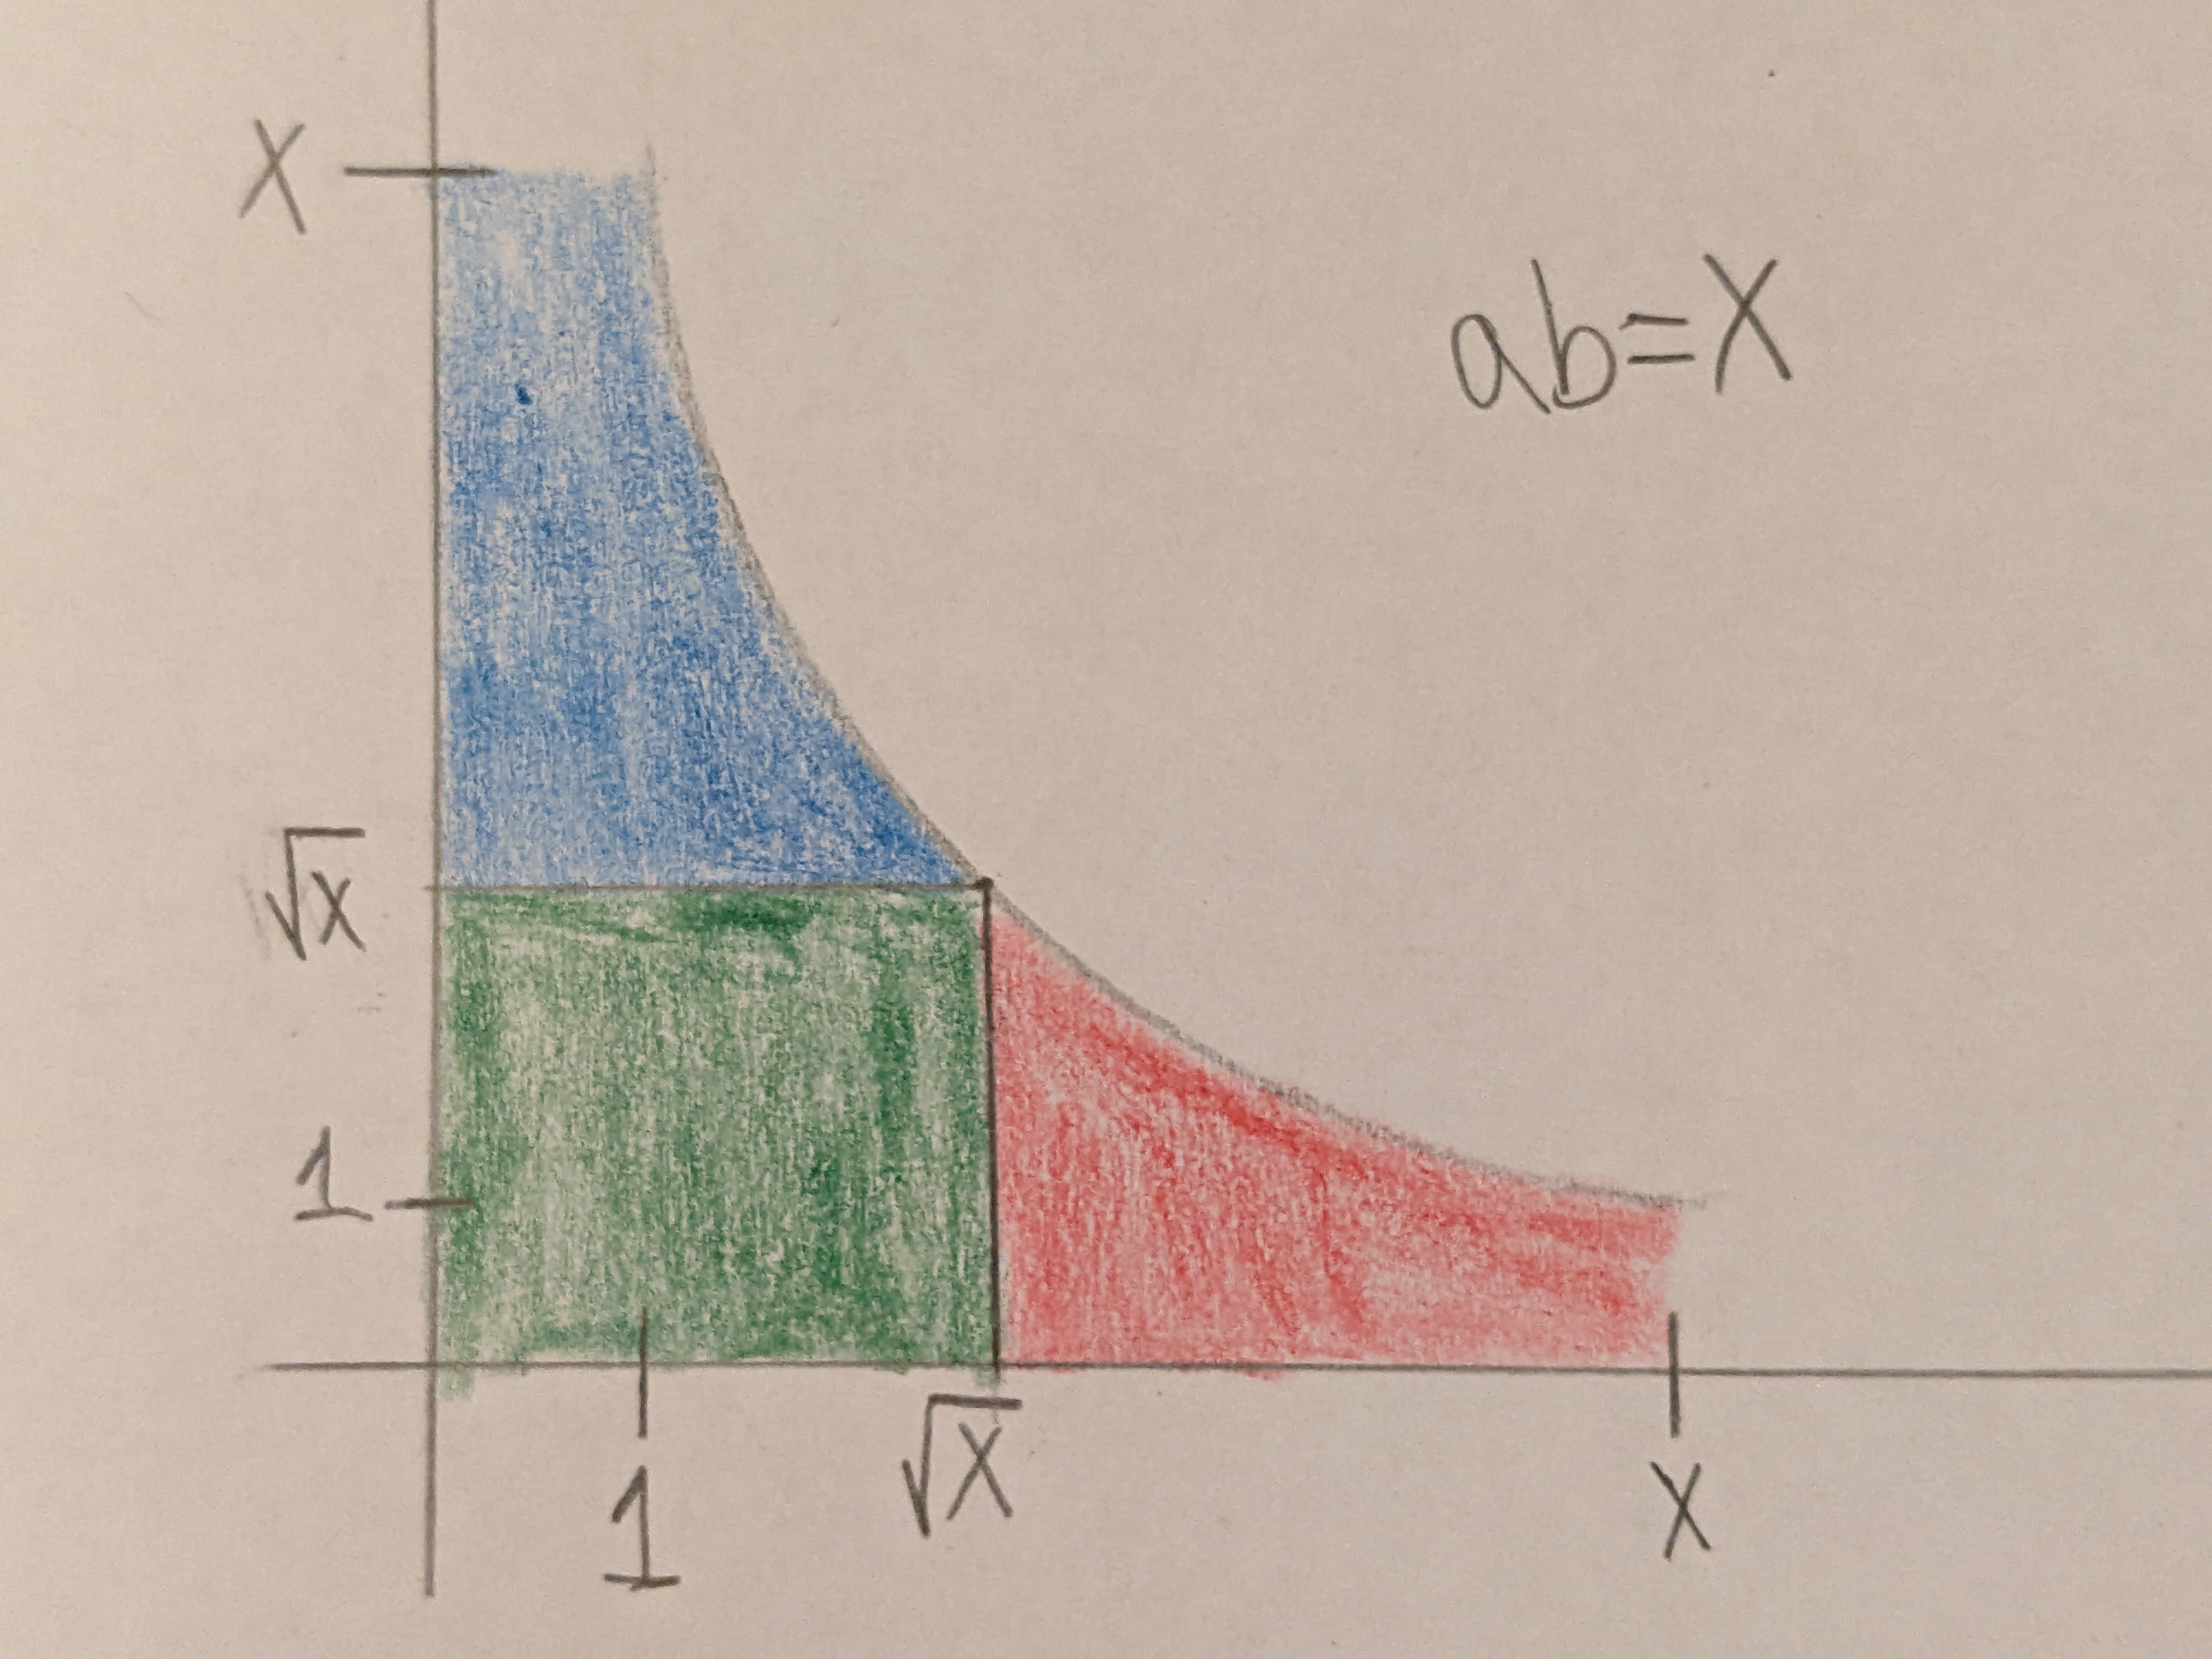
\includegraphics[width=0.8\textwidth]{Problem5Image1}
\end{figure} 
\newpage
\section*{Problem 6}
By Problem $3$, we may suppose without loss of generality that $X$ is an integer. In class, we proved that
\[
\sum_{n \leq X} f(n) \bigg[ \frac{X}{n} \bigg] =  \sum_{n \leq X} g(n)
\] where $f$ is an arithmetic function and $g$ is its mobius transform. Let $f = \mu$, that is, we are letting $f$ equal the mobius function $\mu$. In this case, we have
\[
g(n) = \sum_{d \mid n} f(d) = \sum_{d \mid n}  \mu(d)
\] In class, we proved that $g(n) = 1$ if $n=1$ and $g(n) = 0$ if $n > 1$. By substitution, we find that
\[
\sum_{n \leq X} \mu(n) \bigg[ \frac{X}{n} \bigg] = \sum_{n \leq X} f(n) \bigg[ \frac{X}{n} \bigg] = \sum_{n \leq X} g(n) = 1
\]
\newpage
\section*{Problem 7}
By Problem $3$, we may suppose without loss of generality that $X$ is an integer. In class, we proved that
\[
\sum_{n \leq X} f(n) \bigg[ \frac{X}{n} \bigg] =  \sum_{n \leq X} g(n)
\] where $f$ is an arithmetic function and $g$ is its mobius transform. Let $f = \Lambda$, that is, we are letting $f$ equal the von Mangoldt function $\Lambda$. Then, we have
\[
g(n) = \sum_{d\mid n} f(d) =  \sum_{d\mid n} \Lambda (d) = \log(n)
\] We proved the last equality in class. By substitution, we may deduce that
\[
\sum_{n \leq X} \Lambda(n) \bigg[ \frac{X}{n} \bigg] = \sum_{n \leq X} f(n) \bigg[ \frac{X}{n} \bigg]  =  \sum_{n \leq X} g(n) = \sum_{n \leq X} \log(n)
\]
 \end{document} 